
% !TeX root = ../dissertation.tex

\chapter{Towards a Graphical User Interface for Uppex}

To enhance usability and accessibility, an initial web interface for Uppex was developed, aiming to simplify interaction with the tool and reduce reliance on command-line execution. This interface combines Python (Flask library) on the backend and JavaScript on the frontend to provide a responsive and user-friendly experience. In order to make Uppex a more user-friendly tool for all types of users, initial steps were taken to develop an interface using Python (Flask library) and JavaScript. The proposed frontend was implemented in Python using the Flask library, providing a web-based interface for the uppex.jar verification tool. The application defines routes that enable the loading of model files (XML/IMI), the automatic extraction of configuration parameters from an associated Excel file, and the execution of the different operating modes supported by uppex.jar (--run, --runAll, --validate, --info). The results are then presented directly in the browser, allowing users to interact with the verification engine through an intuitive graphical interface. This approach eliminates the need for command-line interaction, thereby improving usability and reducing the likelihood of user errors.
\medskip

\noindent
\textbf{Requirements.} To be able to use the beta version of the tool, it is necessary to ensure that the following conditions are met: Python, the Java Virtual Machine (JVM), and Bash are installed, and Docker is available.

\medskip

\noindent
\textbf{Installation.} When the conditions above are met, the user can install this GUI by downloading and running the following Bash script:
\url{https://github.com/alexandre04032000/uppex-imitator/blob/Uppex-Imitator/interface.sh}. 
If the process runs successfully, the application will be available on port 8080 of the localhost.

The installation script is designed to automate all necessary steps, including dependency checks, environment setup, and configuration of the server to run the GUI. Users should ensure that they have sufficient permissions to execute Bash scripts and that their system meets the minimum requirements for running the application. After execution, the script will provide output messages indicating the status of each step, such as downloading necessary libraries, setting environment variables, and starting the local server. Once the server is running, users can open a web browser and navigate to \texttt{http://localhost:8080}
 to access the interface.

\medskip

\noindent
\textbf{Running.} This interface allows users to choose between the desired model checker, specifically between Uppaal and IMITATOR. Once one of these options is selected, a menu is displayed (as shown in Figure \ref{fig:UI}), allowing the user to choose from the following options:

\begin{itemize}
    \item Validate the Model
    \item Run a Single Product
    \item Run All Products
    \item Change the Excel File
    \item Change .imi or .xml file
\end{itemize}

\begin{figure}[H]
    \centering
    \begin{minipage}{0.78\textwidth}
        \centering
        \begin{tikzpicture}
            \node[anchor=south west,inner sep=0] (image1) at (0,0) {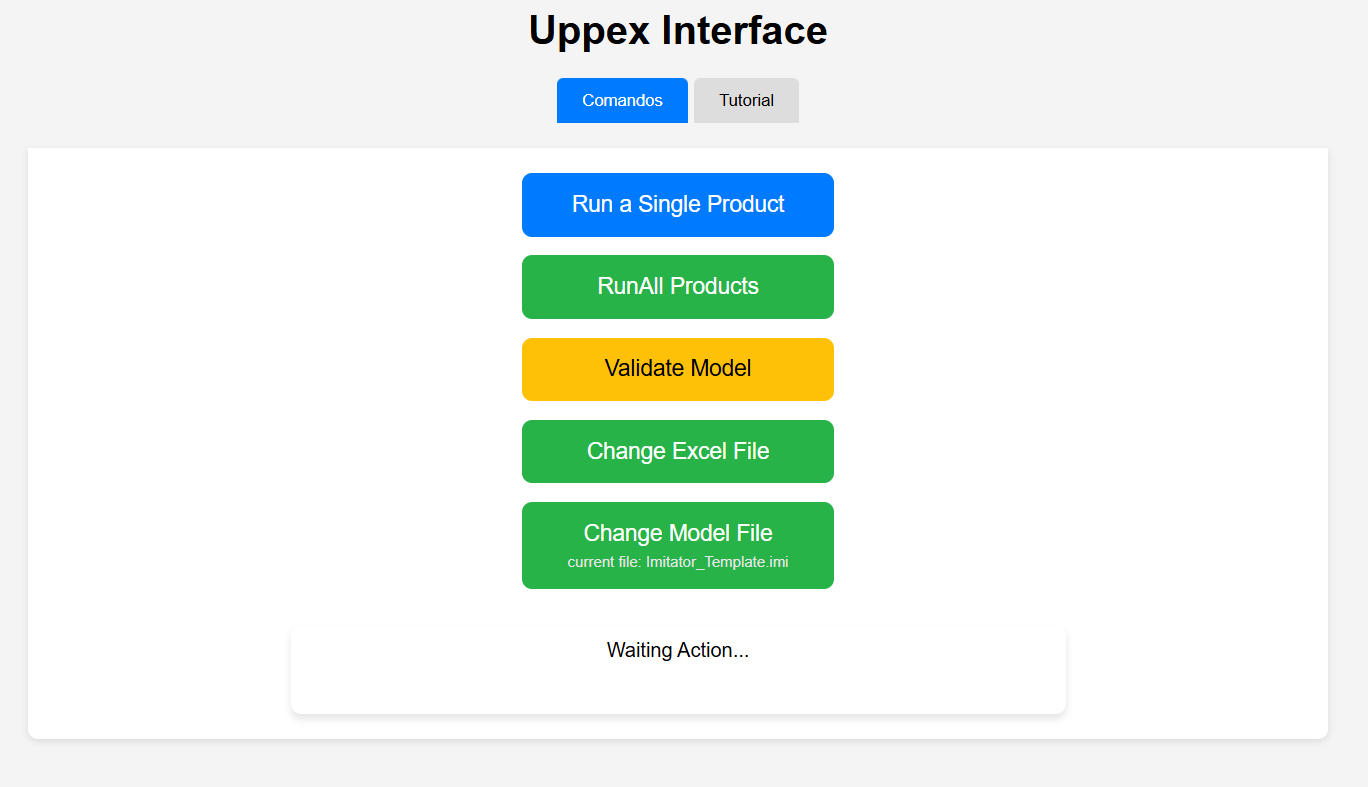
\includegraphics[width=\linewidth]{images/Interface.png}};
            \begin{scope}[x={(image1.south east)},y={(image1.north west)}]
                \draw[black, thick] (0,0) rectangle (1,1); % coordenadas normalizadas
            \end{scope}
        \end{tikzpicture}
        \caption{Uppex Interface Menu}
        \label{fig:UI}
    \end{minipage}
\end{figure}

It should be emphasized that, depending on the choice between Uppaal or Imitator in the menu shown in Figure \ref{fig:UI}, the file extension required for selection is automatically indicated in the final option, which also helps the user identify which file is being read. Additionally, there is a separate tab called \textit{Tutorial}, which, as the name suggests, guides the user step by step in interacting with the tool. Once the model is executed, a PDF report summarizing the results is opened immediately in a separate tab.



